\section{TANDING (Sparring Match) Category}
\label{sec:tanding_category}

\begin{legal}
\item TANDING Equipment:
    \begin{legal}
    \item Attire: \\

Pesilat (contestant) wears a standard black Pencak Silat attire (Figure~\ref{fig:tanding_uniform_front}), the sleeves up till the wrist (+/- 1cm) (Figure~\ref{fig:tanding_uniform_sleeves}) and the length of the pants up to the ankle (+/- 1cm) and a white sash (Figure~\ref{fig:tanding_uniform_pesilat}). \\

For ladies contestant with veil (head cover) it should be in plain black.  During the match white sash must be taken off.\\

It is allowed to have the badge of the contestant’s main association on the left chest and PERSILAT badge on the right chest, the national flag on right arm and sponsor logo on left arm where the size of sponsor logo must not exceed the size of PERSILAT badge (not exceeding 10cm diameter).\\

The name of the country may be printed at the top back of the attire (Figure~\ref{fig:tanding_uniform_back}). All attire must be provided by the individual Pesilat (contestant).\\

The Pesilat does not wear any other accessories except Pencak Silat Attire.\\


    \begin{figure}[h!]
    \centering
    \subfigure[Tanding Uniform Front]{\label{fig:tanding_uniform_front}
        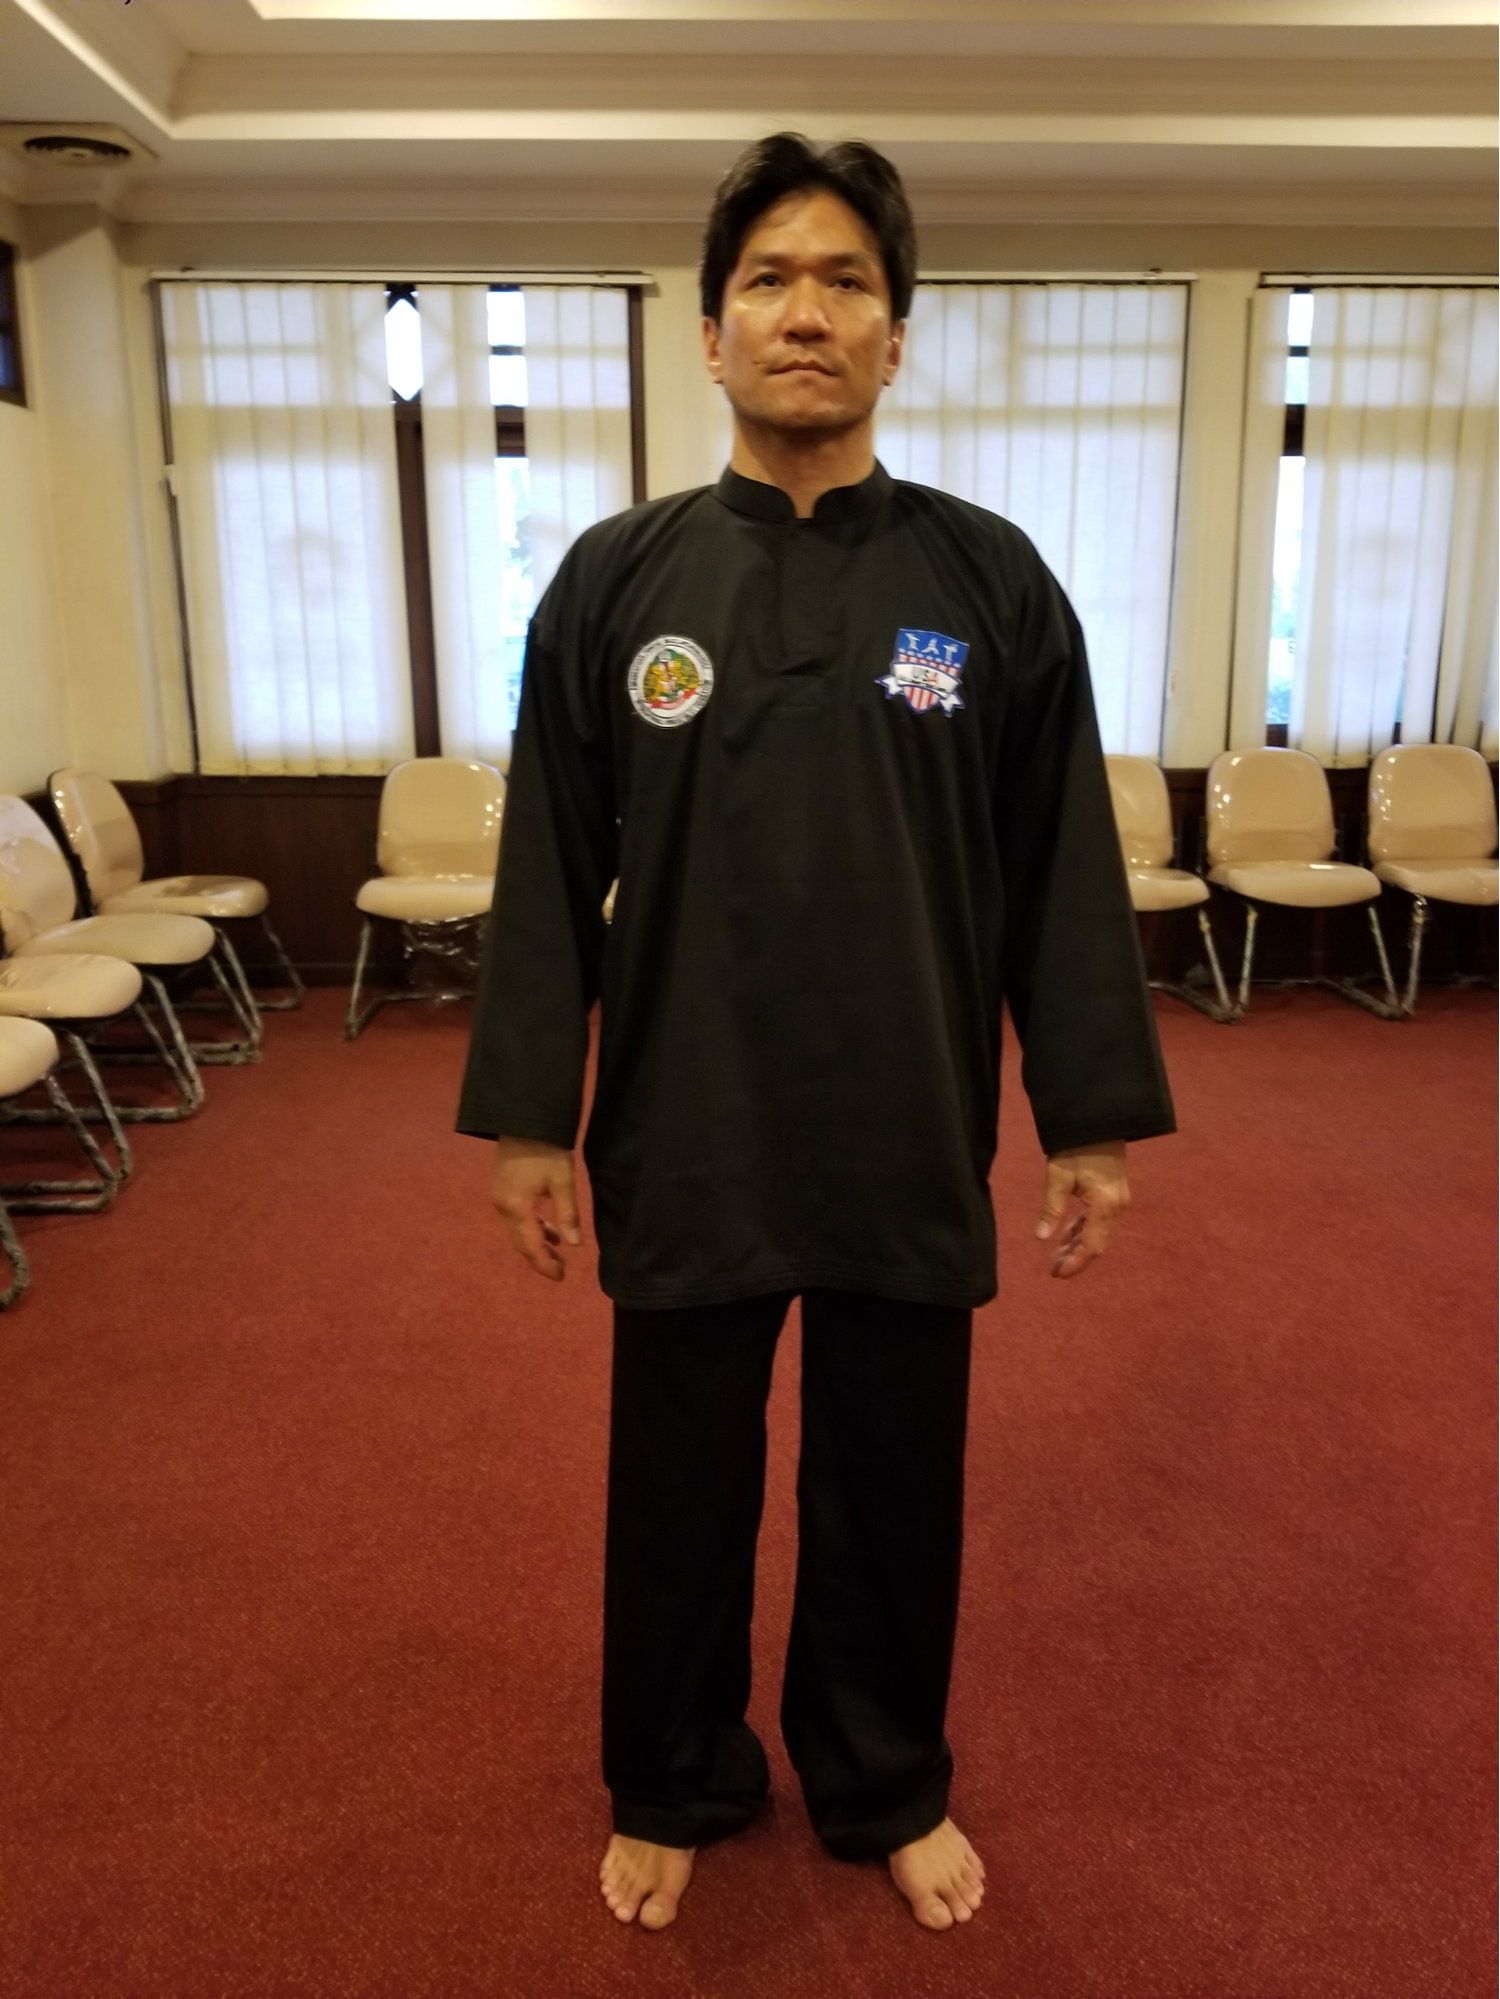
\includegraphics[height=3.0in]{images/tanding_uniform_front}
    }
    ~
    \subfigure[Full Competitor's Tanding Uniform with Sash]{\label{fig:tanding_uniform_pesilat}
        \includegraphics[height=3.0in]{images/tanding_uniform_pesilat}
    }
    \\
    \subfigure[Tanding Uniform Sleeves and Cuff]{\label{fig:tanding_uniform_sleeves}
        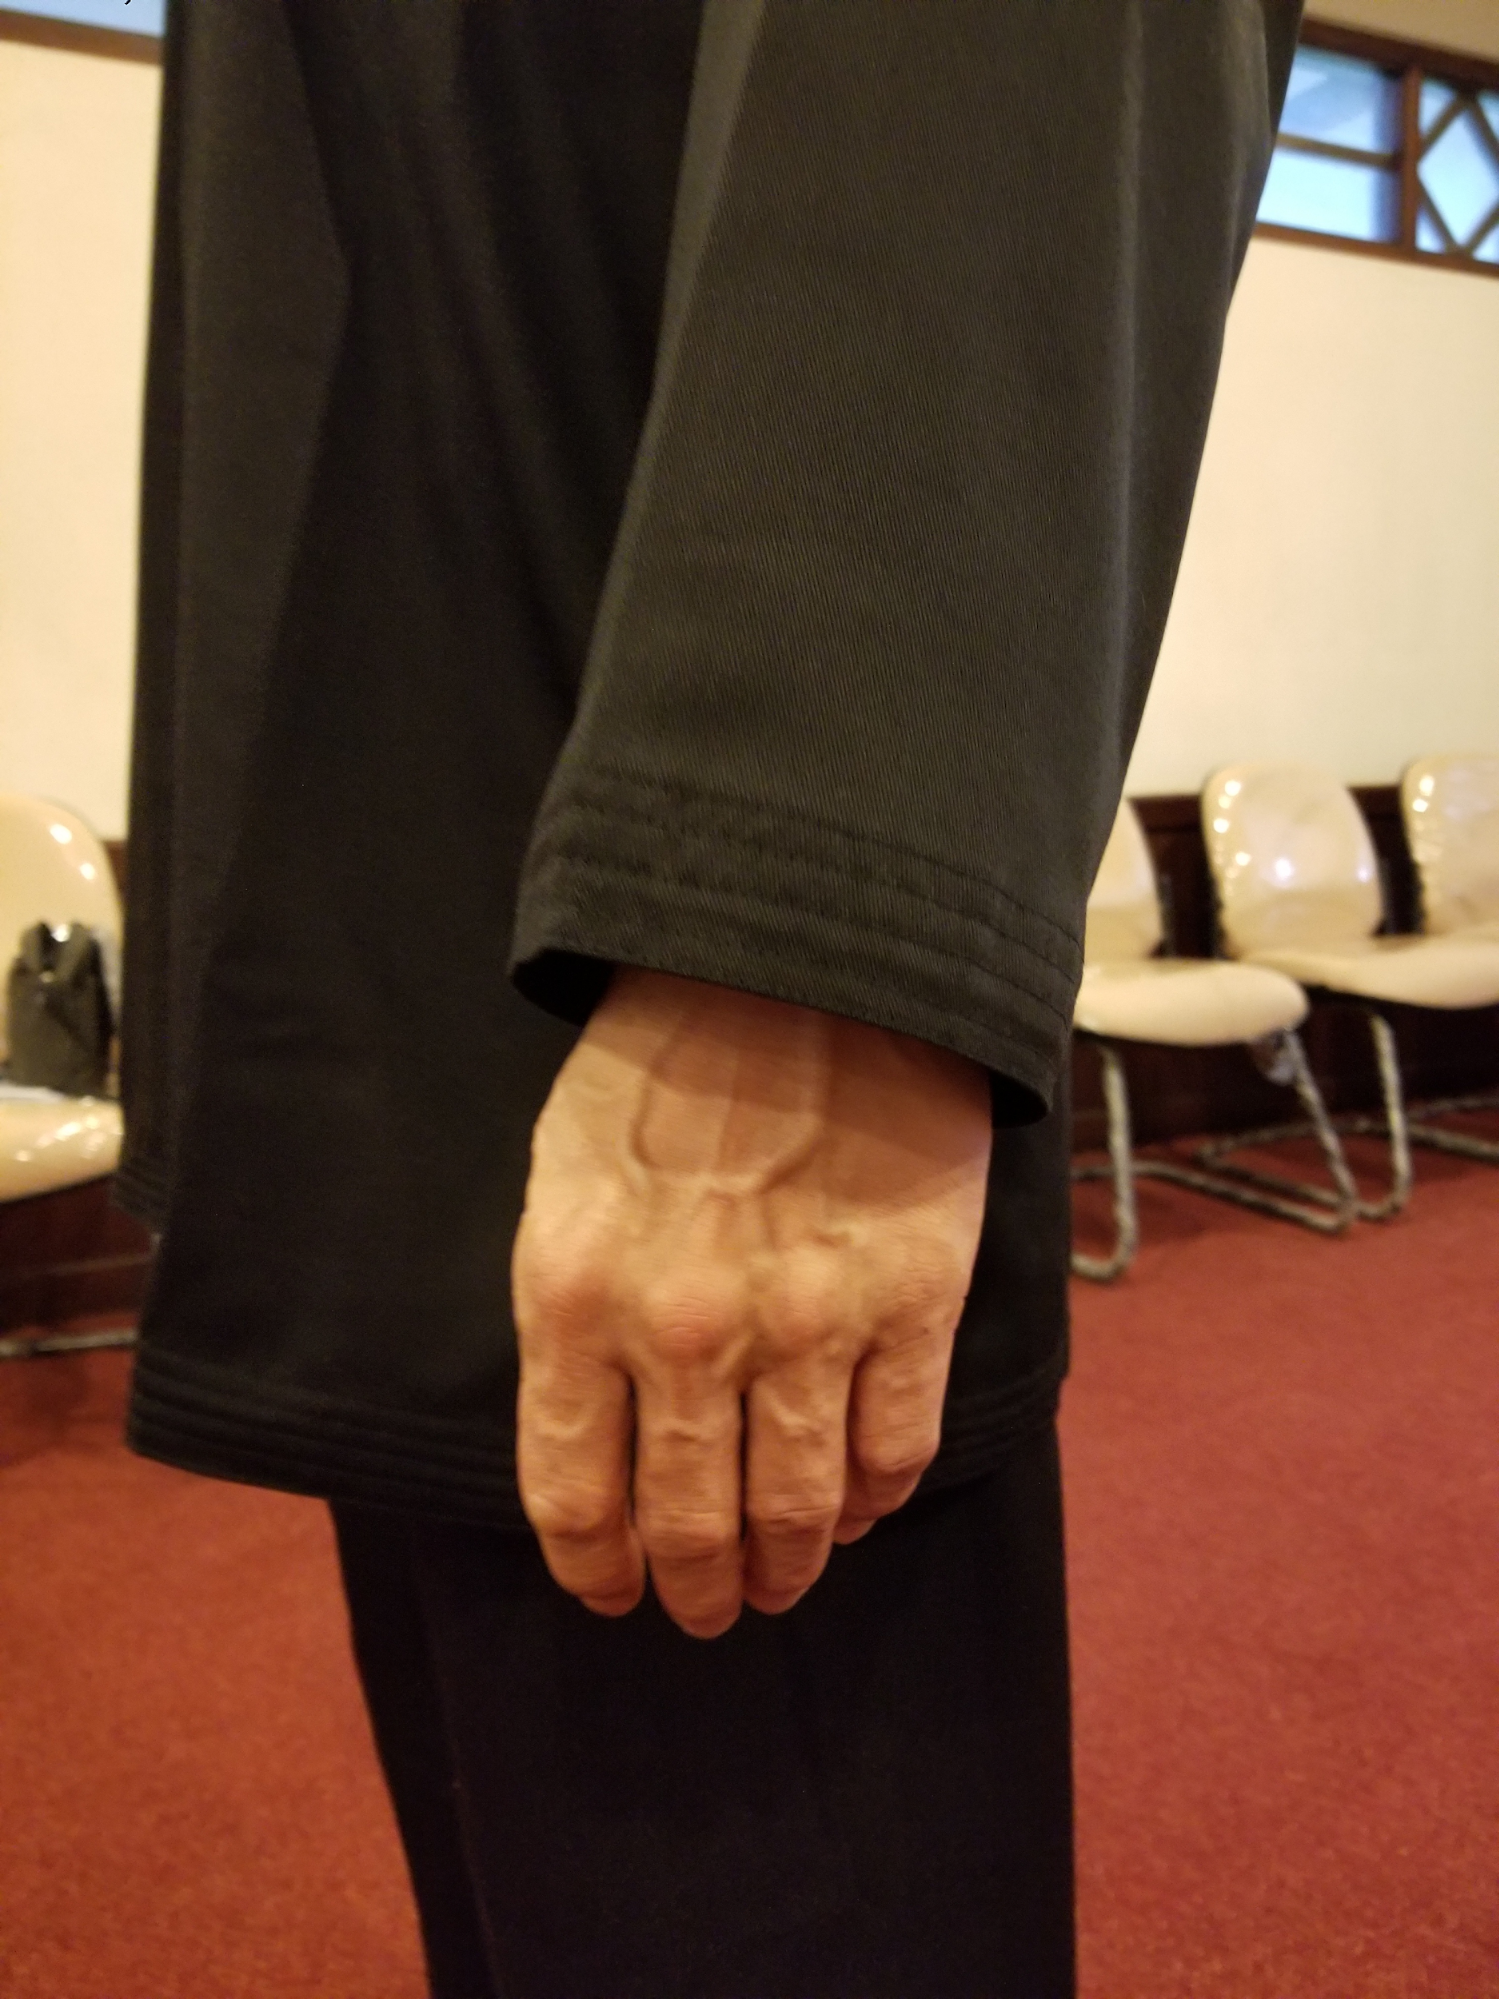
\includegraphics[height=3.0in]{images/tanding_uniform_sleeves}
    }
    ~
    \subfigure[Tanding Uniform Back]{\label{fig:tanding_uniform_back}
        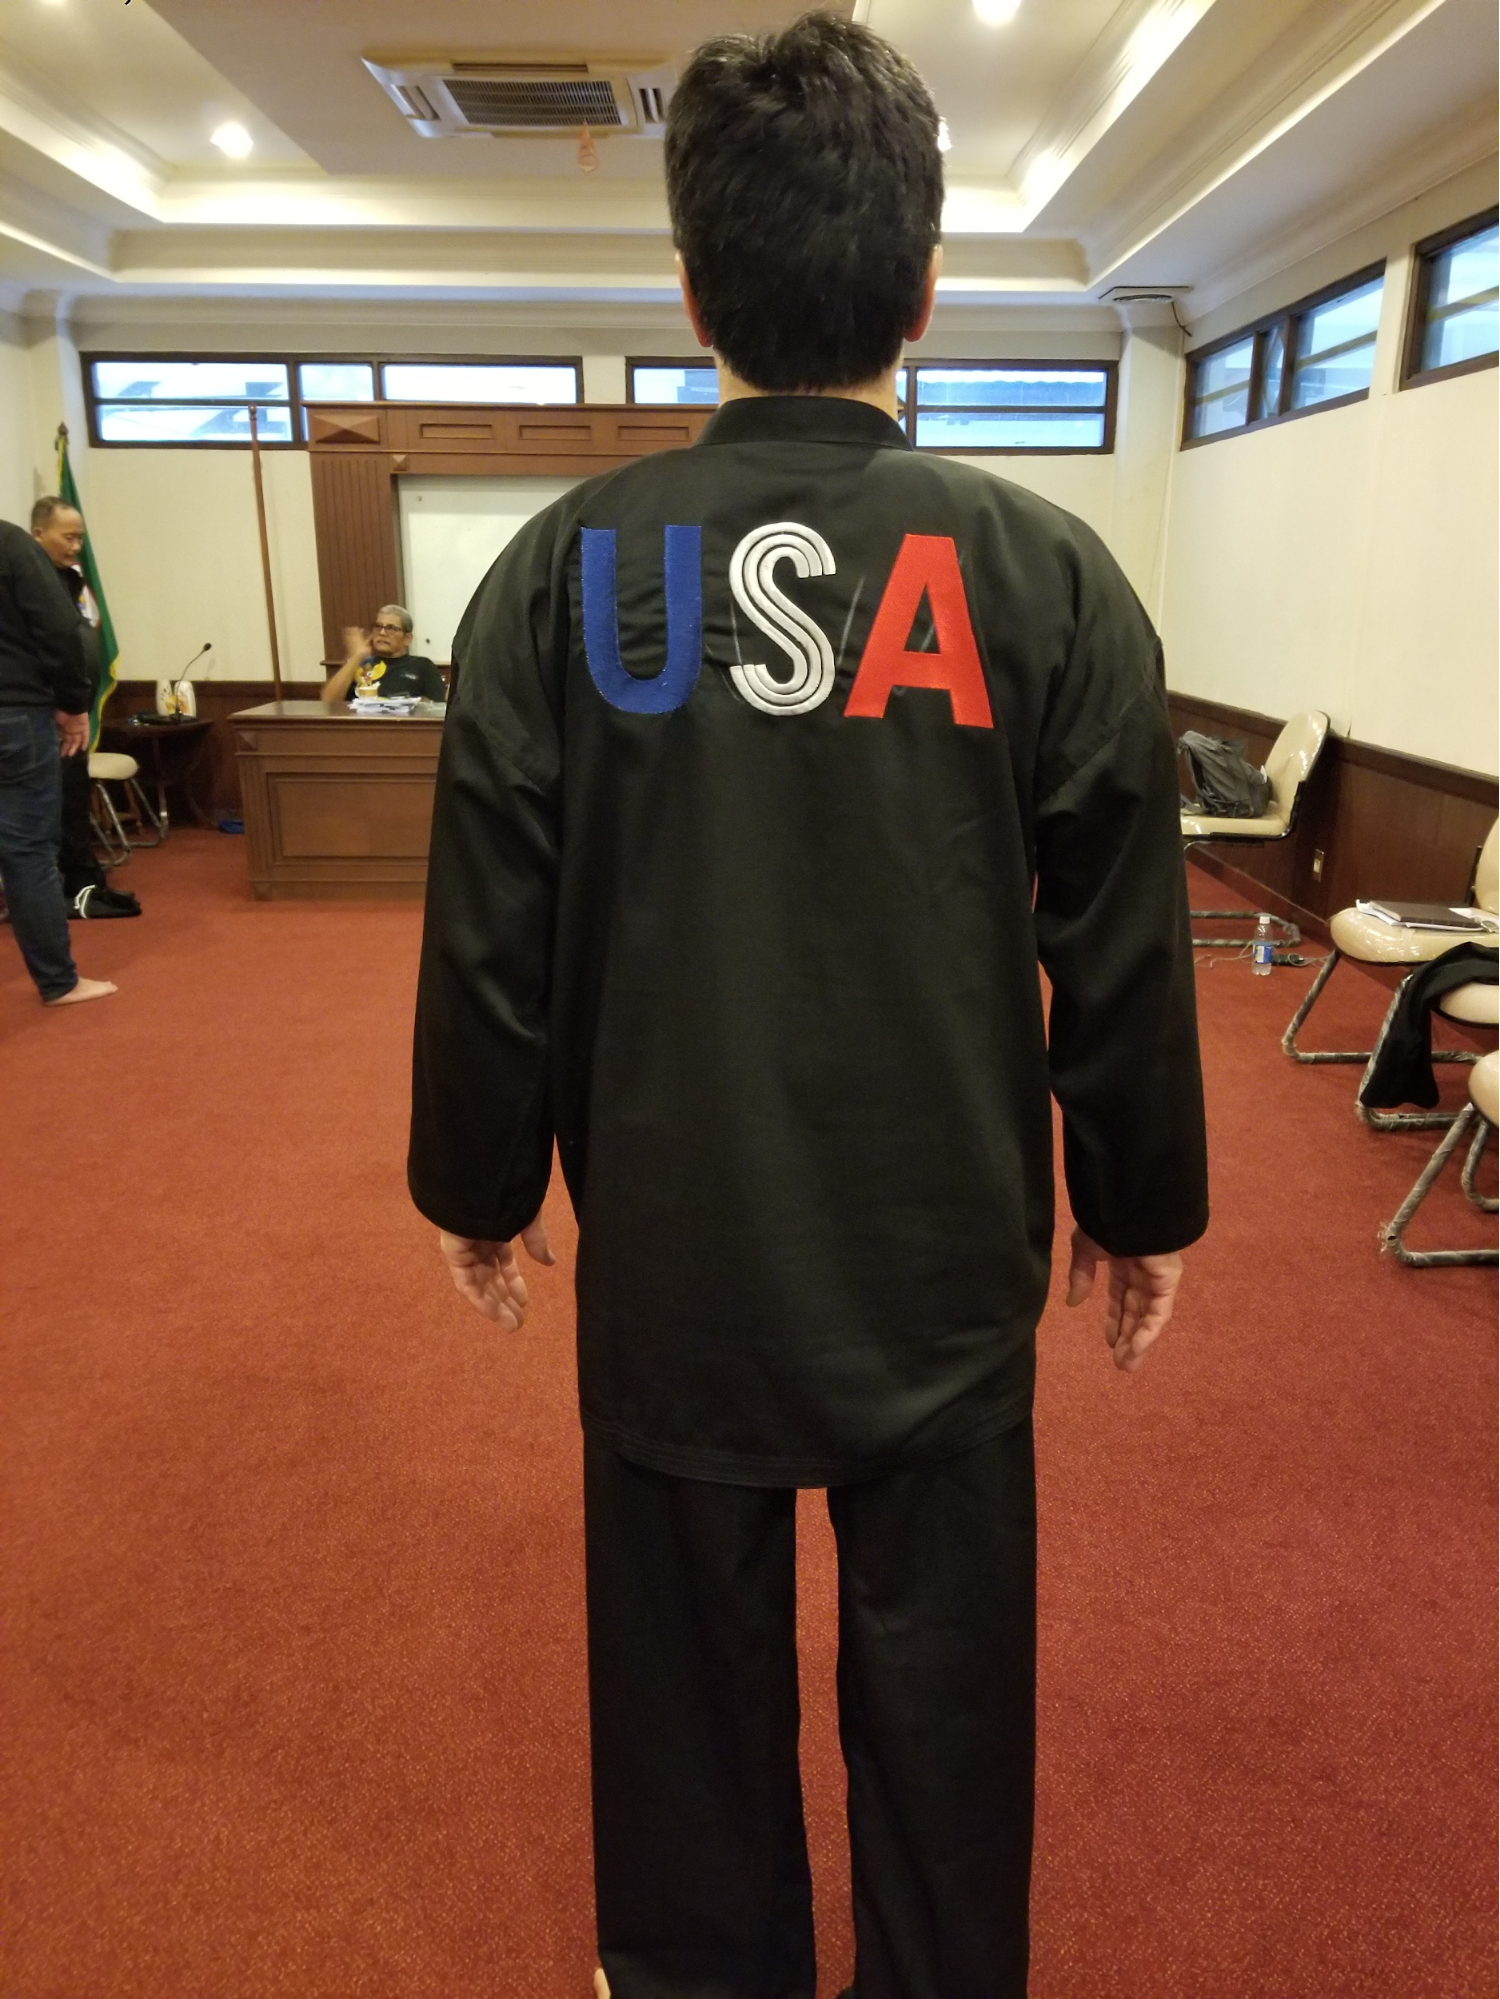
\includegraphics[height=3.0in]{images/tanding_uniform_back}
    }
    \caption{Example Tanding Attire and Details}
    \end{figure}


    \item Body Protector with the following regulations:
    \begin{legal}
        \item PERSILAT quality standard
        \item Black colored
        \item Five sizes: Super Extra Large (XXL), Extra Large (XL), Large (L), Medium (M), and Small (S)
        \item A red or blue sabuk/bengkung (belt/sash) for Pesilat’s corner identification. Size 10cm wide made from uneasy to fold material
        \item One arena should provide at least 5 (five) sets of body protectors of every size that is provided by the Organizing Committee. Mandatory for all athletes to put on the body protectors provided by the Organizing Committee.
    \end{legal}

    \item Groin Protection
    
    It is mandatory for all Male/Female contestants to wear a plastic groin guard provided by the Pesilat (contestant).

    \item Joint Guards

    Joint guards (wrist, ankle, knee, shoulder and elbow), shin and arm guards are allowed to be used in only 1 layer with 1 cm maximum thickness and made from non-hard materials.

    \item Joint Taping is allowed

    \item Mouth guards are allowed
    \end{legal}

\item System and Competition Rounds
    \begin{legal}
    \item Competition uses knock out system. Other systems may be adopted by PERSILAT as and when required.
    \item The competition stages are divided into elimination round, quarter final round, semifinal round and final round, depending on the number of participants. This competition stages shall apply to all classes.
    \item Each competing class should be participated by at least 2 (two) Pesilat (contestants).
    \end{legal}

\item Match Rounds and Time
    \begin{legal}
    \item A match is carried out in 3 (three) rounds. 
    \item Each round takes exactly 2 (two) minutes net. 
    \item Between rounds there is a one-minute net rest.
    \item Moments when the Referee stops the match are not included in the match time. (The counting towards a Pesilat who is knock-downed due to a valid attack is not included in the match time)
    \end{legal}


\item The Pesilat’s Coach
    \begin{legal}
    \item Each Pesilat, particularly in Tanding (Sparring Match) category, is assisted by 2 (two) coaches maximum and understand the Rules and Regulations of Competition of PERSILAT.
    \item The coach’s attire is a PERSILAT standard black Pencak Silat attire (Figure~\ref{fig:tanding_coach}), the sleeves up till
the wrist (+/- 1cm) and the length of the pants up to the ankle (+/- 1cm) with badge
of his/her main association on the left chest and is allowed to put PERSILAT badge on
the right chest, name of the country on the back and wears an orange sash of 10-cm wide.
    \item The coach is allowed to give advice only during rest between rounds.
    \item One of the coaches must be of the same gender with the Pesilat (contestant).

    \begin{figure}[t!]
        \centering
        \subfigure[Coach]{\label{fig:tanding_coach}
            \includegraphics[height=2.5in]{images/tanding_coach}
        }
        ~
        \subfigure[Wasit (Referee) / Judge (Juri)]{\label{fig:tanding_wasit_juri}
            \includegraphics[height=2.5in]{images/wasit_juri}
        }
        ~
        \subfigure[Competition Chairperson]{\label{fig:tanding_chairperson}
            \includegraphics[height=2.5in]{images/chairperson}
        }
        \caption{Competition Officials}
    \end{figure}
    \end{legal}

\item Competition Procedure
    \begin{legal}
    \item The competition is commenced by the Referee and Jury \ref{fig:tanding_wasit_juri} 
    entering the arena from the
    right side of the Competition Chairperson \ref{fig:tanding_chairperson}. 
    Before entering the arena Referee and Jury bow and report to the 
    Competition Chairperson that they are ready to carry out their duties.
    \item Referee shall check the athlete at their individual corners before commencing the
    match. At Referee’s signal, each Pesilat enters the arena from his/her corner,
    bowing/signal respecting to the Coaches, Referee and the Competition Chairman. Afterwards each
    Pesilat is required to perform 5 (five) to 10 (ten) school’s movement (jurus
    perguruan) before returning to their respective corners.
    \item The match will commence by the Referee calling both Pesilats. The Pesilats will then
shake hands, reminding on the rules and be ready for the match.
    \item After the Referee checks the readiness of all officials by means of right hand signal,
he commands both Pesilats to begin the match.
    \item During break time, both Pesilats must return to their respective corners.
    \item Beside the Referee and the two contestants, no one else may enter the arena unless
otherwise, upon the Referee’s request.
    \item At the end of the final round, both Pesilats return to their respective corners to wait
for the decision of the winner. By the time to announce the winner, Referee calls both
Pesilats to the center of arena. Upon announcement of winner, Referee will lift the
winner’s hand. After that both Pesilat respect the Competition Chairman.
    \item After paying respect, both Pesilat’s shake hands and leave the arena. The Referee and
Jury shall come forward in front of the Chairman and give respect, and report to the
Competition Chairman about the completion of their duties. The Referee and Jury
leave the area via the left side of Competition Chairman’s table.
    \end{legal}

\item The Rules of the Game:
    \begin{legal}
    \item The Rules of the Game:
        \begin{legal}
        \item The Pesilats confront each other by applying the Pencak Silat defense and attack
              elements ie. Repulsing, dodging, hitting the target, dropping the opponent; and
              complying to the Pencak Silat Rules and Regulations.
        \item  By applying the `\emph{Pencak Silat principle}', it means to obtain technical scores, a Pesilat
               must apply a combative pattern which consists of on-guard position (sikap-pasang),
               step pattern (pola langkah, Figure~\ref{fig:pola_langkah}), maintain the distance 
               against the opponent, while
               performing the attack/defense, and finally return to the on-guard position (sikap
               pasang, see Figure~\ref{fig:sikap_pasang}).

            \begin{figure}[t!]
                \centering
                \includegraphics[width=4.0in]{images/pola_langkah_dasar}
                \caption{Example Footwork Patterns (Pola Langkah)}
\label{fig:pola_langkah}
            \end{figure}

            \begin{figure}[ht!]
            \centering
            \subfigure[]{\label{fig:sikap_pasang_1}
                \includegraphics[height=1.5in]{images/sikap_pasang_1}
            }
            ~
            \subfigure[]{\label{fig:sikap_pasang_2}
                \includegraphics[height=1.5in]{images/sikap_pasang_2}
            }
            \subfigure[]{\label{fig:sikap_pasang_3}
                \includegraphics[height=1.5in]{images/sikap_pasang_3}
            }
            ~
            \subfigure[]{\label{fig:sikap_pasang_4}
                \includegraphics[height=1.5in]{images/sikap_pasang_4}
            }
            \caption{Example Sikap Pasang}
            \label{fig:sikap_pasang}
            \end{figure}


 
        \item Defense and/or attack must start from on-guard position (sikap pasang),
        followed by a step pattern (pola langkah), with demonstration of good coordination in
        performing an attack defense.  After performing an attack/defense, Pesilat must return on to 
        the on-guard applying step pattern. The Referee will give command `\emph{Langkah}' if a Pesilat 
        does not use proper technique of Pencak Silat.
        \item A series of attacks should be delivered in row, a combination of various
        techniques towards the target, with not more than 6 (six) techniques of attacks, per
        exponent. A Pesilat who performs more than 6 (six) techniques of attacks in a row will
        be stopped by the Referee.  
        Continuous attacks with the hand using the same technique will only score 1 point.
        \item An attack that scores points hits the target by applying the principles and 
        is stable and powerful.
        \end{legal}

        \item Competition Commands
        \begin{legal}
        \item The command `\emph{BERSEDIA}' (Get Ready) is used to alert both Pesilat and 
        all competition officials to be ready as the match is about to begin. The command shall
        be used throughout the match.  Approximate English pronunciation \emph{burr-said-E-ah}.
        \item  The command `\emph{MULAI}' (Start) is used each time a match is started or continued.
This command is used together with the hand signal.  Approximate English pronunciation: \emph{moo-lie}.
        \item The command `\emph{BERHENTI}' (Stop) or `\emph{TI}' is used to stop the match.  Approximate English pronunciation: \emph{burr-hen-tee}.
        \item The commands `\emph{PASANG}', `\emph{LANGKAH}', and `\emph{SILAT}' are used to give guidance.  Approximate English pronunciations: \emph{paw-song}, \emph{long-caw}, \emph{see-lot}.
        \item The start and the end of each round is marked by a strike on the Gong.
        \end{legal}


    \item Targets\\
    A target is defined as the valid areas for attacking for which points can be awarded.  They
    are on the body covering the trunk area excluding the neck and upwards and the navel to the groin.
    Figure~\ref{fig:attacking_targets} illustrates some of the following targets:
        \begin{legal}
        \item Chest
        \item Abdominal (navel upwards)
        \item Left and right ribs
        \item Back part of the trunk (except direct attack to the whole spinal cord)
        \\
    The lower limb (ankle and below) can be targeted for an intercepting attack while aiming to
    drop the opponent but is a non-scoring area.

        \begin{figure}[h!]
            \centering
            \includegraphics[width=4.0in]{images/attacking_targets}
            \caption{Valid Attacking Targets}
            \label{fig:attacking_targets}
        \end{figure}

        \end{legal}
    
    \item Prohibitions \\
    Prohibitions which are declared as violations:
        \begin{legal}
        \item Serious violations
            \begin{enumerate}[label=\alph*.]
            \item Attack illegal parts of body ie. Neck, head and navel downwards to groin,
            direct attack to the whole spinal cord, thigh and lower limbs shin area.
            \item Direct attempts to break the joints.
            \item Deliberately throw the opponent out of the arena
            \item Attack with head (Head Butt)
            \item Attack the opponent before the `\emph{MULAI}' command or after the `\emph{BERHENTI}'
            command is given by the Referee, causing injury to the opponent.
            \item Wrestle, bite, scratch, grip, and pull the opponent’s hair/jilbab (pull hair/jilbab)
            \item A Pesilat challenges, humiliates, hits, utters vulgarities, spits, shouts to
                  provoke opponent or Competition Officials (Technical Delegate,
                  Competition Chairman, Council of Referee-Jury, Referee-Jury and all other
                  officials on duty), and to all spectators.
            \item Slamming down the opponent in or out of arena within the match period.
            \item Gripping, grabbing or embrace while attacking.
            \end{enumerate}

        \item Light violations
            \begin{enumerate}[label=\alph*.]
            \item Does not use on-guard position and step pattern.
            \item Walks out of the arena (any one leg out of the arena) whether intentionally
                  or unintentionally more than 1 (one) time in 1 (one) round
            \item Embrace the opponent in process of defending
            \item Attack with front/back sweeping technique, scissoring while in lying
                  position more than 1 (one) time in 1 (one) round to waste time.
            \item Communicate with outside or coaches either by certain gesture/signals or
by spoken words
            \item Both Pesilats are passive or when one of Pesilat is passive more than 5
seconds.
            \item  Shouting during competing.
            \item Wrong direction of attack.
            \item Intentionally push the opponent out of the arena.
            \item Athlete that turns his/her back against the opponent to waste time or
                  prevent an attack.
            \item Time delaying tactics (releasing the body protector knot, untying of the
hairband, was given the counting etc)
            \end{enumerate}

        \end{legal}

    \item Improper Defense Technique
        \begin{legal}
        \item A valid attack with accurate direction but may cause injury to the opponent 
             due to improper defensive technique (i.e.\ dodging towards the incoming attack)
             direction is not a violation.
        \item If the attacked Pesilat is injured, the Referee will call for the doctor
              immediately. If the doctor decides that the injured Pesilat is unfit to continue fighting,
              the Pesilat will be declared defeated by `technical knock-out' (TKO).
        \item If the doctor declares that the injured Pesilat is fit to continue, but he/she fail
              to stand up at once, the Referee will immediately start the technical counting.
        \end{legal}

    \item Penalties\\
    Level and types of penalties
        \begin{legal}
        \item Reprimand
            \begin{enumerate}[label=\alph*.]
            \item Given when a Pesilat commits light violation after 1 (one) time verbal warning of
                  the same violation within the same round.
            \item Reprimand can directly be given when a Pesilat commits severe violation without
                  causing injury to the opponent.
            \end{enumerate}

        \item Warnings shall be valid for all rounds only for severe violations. 
              For light violation, it ends at every round, consist of:
            \begin{legal}
            \item Warning I \\
            Warning I is given when a Pesilat:
                \begin{enumerate}[label=\alph*.]
                \item Commits severe violation causing injury to opponent
                \item Given third reprimand as the result of light violation
                \end{enumerate}

            After Warning I is given, another reprimand will be given for another type of
            violation within the same round.

            \item Warning II \\
            Warning II is given when a Pesilat commits another severe violation after Warning I.
            Warning II is given, another reprimand will be given for another type of light
            violation within the same round.

            \item Warning III \\
            Warning III is given when a Pesilat commits another severe violation after

            Warning II and will be immediately disqualified.

            Warning III should be shown by the Referee.

            \item Disqualification \\
            Is given when a Pesilat:
                \begin{enumerate}[label=\alph*.]
                \item commits another severe violation after Warning II.
                \item commits serious violation deliberately and contradicts against the
                      sportsmanship.
                \item commits serious violation which receives Warning I or Reprimand
                      I, and the injured opponent is unfit to continue the match as per officiating
                      Doctor’s decision.
                \item fails to meet the weight requirement during the second weigh-in conducted 15
                      minutes before the match.
                \item fails the doping test. A Pesilat that fails the doping test will be
                      disqualified. All medals, certificates and all other awards shall be returned
                      to the Organizing Committee.
                \item is unable to provide the letter of medical checkup before starting the
                      first match (regardless of category) of the competition.
                \end{enumerate}
            \end{legal}


        \end{legal}

        \item Scoring\\

            \begin{legal}
            \item Scoring Rules \\
        \begin{table}[h!]
        \centering
        \begin{tabular}{l|ll}
        Total     & \multicolumn{2}{l}{Breakdown} \\
        \hline
        Score +1  & +1  & An attack by hand/elbow successfully hitting the target without being blocked \\
        \hline
        Score +2  & +1  & Successfully voiding opponent’s attack \\
                  & +1  & AND immediately followed by a successful counter attack by hand. \\
        \hline
        Score +2  & +2  & An attack by foot/knee successfully hitting the target without being blocked. \\
        \hline
        Score +3  & +1  & Successfully voiding opponent’s attack \\
                  & +2  & AND immediately followed by a successful counter attack by foot. \\
        \hline
        Score +3  & +3  & Direct attack that successfully drops the opponent. \\
        \hline
        Score +4  & +1  & Successfully grabbing the opponent's leg \\
                  & +3  & AND immediately followed by a successful dropping technique.\\

        \end{tabular}
        \caption{Technical performance score breakdown}
        \label{tbl:tanding_technical_score}
        \end{table}

            \item Qualifications of Technical Score: (valid scoring) \\
                  Valid score shall be given to the following:
                \begin{enumerate}[label=\Alph*.]
                \item Blocking or evading followed by an immediate valid counter attack
                \item Valid hand attack
                \item Valid foot attack
                \item Valid dropping technique
                \end{enumerate}
                
                \begin{enumerate}[label=\Alph*.]
                \item Blocking or evading -– successfully void the opponent’s attack followed
                      with immediate valid counter attack, either with the foot, hand or
                      dropping attack. \\
                Note: The score of ``1+'' shall be given for successfully voiding the
                      opponent’s attack followed with immediate valid counter attack, either
                      with the foot, hand or dropping attack. Whereby a direct successful
                      attack shall be given points as per its mode: 1 point = hand attack (direct elbow), 
                      2 points = foot attack (knee) and 3 points = valid drop. (no points shall be given
                      for any blocking or evading without counter attack)
                \item Valid hand attack – all types of hand attack which is direct and powerful.
                      (punches from; front, spade, uppercut, side hook and elbow): +1 point
                \item Valid foot attack – all types of foot attack which is direct and powerful.
                      (kicking techniques; frontal, spinning back, side, half-turn, stomping and knee): +2 points
                \item Valid dropping – all applicable techniques to drop the opponent
                      ensuring that the knee and above touches the floor: +3 points
                    \begin{enumerate}[label*=\arabic*.]
                    \item Applying the direct attack such as sweeping, scissors and lifting with the leg.
                    \item Applying indirect dropping technique by catching of opponent’s
                        leg followed by a valid drop (no punching or kicking at this stage).
                    \item Does not drop together with opponent while applying the valid drop technique.
                    \item Dropping process is given duration of 5 seconds before the Referee stops the fight.
                    \item It is not allowed to wrestle before the techniques; sweeping
                        side drop, lifting with the leg or scissors is used. However,
                        pushing or touching is allowed within the body area.
                    \item A counter attack is allowed when a failed sweeping technique
                        occurs. The score for the counter attacks is determined by the
                        technique applied, without using the body weight within one
                        second period.
                    \end{enumerate}
                \item Other factors in the competition
                    \begin{enumerate}[label*=\arabic*.]
                    \item Concurrent attack is an attack (whether valid or invalid, since
                        those attacks happened accidentally) where one or both of
                        Pesilat fall down, the dropping will be validated by the following criteria:
                        \begin{enumerate}[label*=\arabic*.]
                        \item If one of them is not able to get up, counting will be applied immediately.
                        \item If both of them are not able to get up at once, counting will be applied 
                            immediately to both of them.
                        \item If both Pesilats are not able to get up by count of ten (10),
                            however, both had gained points, the winner will be the one
                            with the highest score.
                        \item If the incident occurs during the beginning of the first
                            round and neither of them gains a score, the decision of the
                            winner according to Chapter~\ref{chp:rules_of_the_game} \ref{sec:tanding_category} point~\ref{pt:victory_decision} \ref{pt:tanding_tie_weight} and \ref{pt:tanding_tie_coin} (no rematch).%article 9 point 6.7.4 a.2_iv and v.  (no rematch).
                        \end{enumerate}
                    \end{enumerate}

                \item Accidental Fall – When a Pesilat falls not because of the opponent’s
                    attack, and not able to get up, he will be given the chance to get up
                    within 10 seconds counting. If the Pesilat is not able to continue the
                    fight, will be declared as lost by `TKO'.

                \item Catching
                    \begin{enumerate}[label*=\arabic*.]
                    \item Catching in a process of dropping an opponent is declared failed when:
                        \begin{enumerate}[label*=\arabic*.]
                        \item The dropping process takes more than 5 (five) seconds, or 
                            dragging/wrestling occurs.
                       \item The attacking Pesilat falls down together in the dropping process.
                        \item If during the dropping process, the caught opponent grabs the shoulder of the 
                           Pesilat trying to drop him/her down, and succeed to drop the him/her within 
                            5 (five) seconds before the Referee gives the command `\emph{BERHENTI}' (stop); 
                            the dropping will be declared as valid.
                        \item If the defending Pesilat touches the neck or head or tugging, causing both 
                            Pesilats to fall down, the tugging Pesilat will be given the `\emph{Teguran}' 
                            (reprimand).
                        \end{enumerate}
                    \end{enumerate}

                \item Dropping
                    \begin{enumerate}[label*=\arabic*.]
                    \item When dropping technique is successful, at least part of the body
                       is inside the arena’s boundary line, the dropping will be
                        declared `valid'.
                    \item When a dropping technique is successful within the arena, and
                        the dropped Pesilat shifts out of the arena the dropping will be
                       declared valid.
                    \item  When a valid attack causes the opponent to fall, and unable to get 
                        up immediately, and within the arena, but the dropped Pesilat shifted himself/herself 
                        out of the arena; valid drop signal shall be given immediately. The dropped Pesilat 
                       will be given chance to stand-up and be on-guard position within 10 (ten) seconds, 
                        failing which the dropped Pesilat is unable to continue the bout, he/she will be 
                        declared losing by TKO.
                    \end{enumerate}
                \end{enumerate}

            \item Penalty

            The progression of point deductions for a penalty are:
                \begin{enumerate}[label*=\arabic*.]
                \item Score -1 (minus 1) is given when a Pesilat gets Reprimand I
                \item Score -2 (minus 2) is given when a Pesilat gets Reprimand II
                \item Score -5 (minus 5) is given when a Pesilat gets Warning I
                \item Score -10 (minus 10) is given when a Pesilat gets Warning II
                \end{enumerate}


            \item Victory Decision \label{pt:victory_decision}
                \begin{enumerate}[label=\alph*.]
                \item Win by Points Score
                    \begin{enumerate}[label*=\arabic*.]
                    \item When a majority of the Juries decides in favor of one Pesilat over another
                        than the opponent.
                    \item In the event where there is a tie, the winner will be determined base on the 
                        following:
                        \begin{enumerate}[label=\roman*.]
                        \item With the least penalty scores
                        \item With the most technical scores binned and prioritized as follows: 
                            1+3, 3, 1+2, 2, 1+1, 1
                        \item An additional round
                        \item \label{pt:tanding_tie_weight} The Pesilat who is lighter (body mass) referring to the weight taken at the re-weighing process, 15 minutes before the game.  and witnessed by Technical Delegate and both team managers
                        \item \label{pt:tanding_tie_coin} A coin toss coins to be carried out by the Chairman of Competition and witnessed by Technical Delegate and both team managers
                        \end{enumerate}

                    \item The Jury’s scores shall be displayed on the scoreboard, at the end of the final
                        round, after the winners decision was announced, except if digital scoring system
                        us used (where the scores will be shown in the screen automatically).
                    \end{enumerate}

                \item Win by Technical Knock Out (TKO) of Opponent is declared winning by 
                    Technical Knock Out when:
                    \begin{enumerate}[label=\arabic*.]
                    \item Opponent requests not to continue the fight.
                    \item Competition Doctor’s decision. Competition Doctor is given 120 (One hundred
                        and twenty) seconds to decide whether Pesilat is declared ‘Fit’ or ‘Unfit’ to
                        continue the fight and to give medical help.
                    \item Coach’s request (throw in towel).
                    \item Referee’s decision. (Upon counting of Pesilat to the count of 10).
                    \end{enumerate}

                \item  Win by Absolute Victory\\
                    The decision of absolute victory is made when the opponent is knocked down due to
                    valid attack and he/she is unable to get up immediately and or feels dizzy or unable to
                    stand upright with `sikap pasang' after Referee’s counting up to 10.

                \item Win by RSC (Referee Stop Contest). \\
                    Winning as the referee deems the bout is unbalanced.

                \item Win by WO (Walkover) \\
                    The opponent did not show up in the arena after the third call, with the interval of 30
                    seconds at each call. Unless the Team Manager had informed the withdrawal of the
                    Pesilat.

                \item Win by Disqualification: \\
                    \begin{enumerate}[label=\arabic*.]
                    \item The opponent gets Warning III after Warning II
                    \item The opponent commits a serious violation and is directly punished with disqualification
                    \item The opponent commits a severe violation injuring the opponent hence he/she is not able
                        to continue, and to be decided by the competition’s doctor. A Pesilat who won by
                        disqualification by this rule, will only be allowed to compete in the next match,
                        with the permission and recommendation from competition’s doctor before the
                        next match.
                    \item During weighing, the Pesilat’s weight does not meet the weight requirement.
                    \item Pesilat failed to show the medical certification before the competition started.
                    \end{enumerate}

                \end{enumerate}
            \end{legal}
    \end{legal}
\end{legal}


